\section{Circuito RLC}

\subsection{Conceito}

Um circuito RLC é um circuito elétrico composto de um resistor (R), um indutor (L), e um capacitor (C), conectados em série ou em paralelo.

É um \textbf{circuito de 2° ordem}, pois qualquer tensão ou corrente nele pode ser descrita por uma equação diferencial de segunda ordem.

\begin{figure}[H]
	\centering
	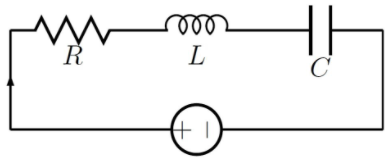
\includegraphics[width=0.8\textwidth]{./Imagens/RLC/rlc1.png} 
	\caption{Desenho esquemático de um circuito RLC}
	\label{fig:RLC1}
\end{figure}

\subsection{Indutor}

Um indutor é um componente eletrônico passivo capaz de armazenar energia elétrica na forma de \textbf{energia magnética}. Basicamente, é constituído de um condutor que é enrolado em uma bobina, e quando a eletricidade flui para a bobina da esquerda para a direita, isso gera um campo magnético cujo sentido pode ser obtido pela regra da mão direita.

O indutor no esquema é usado para representar as características físicas do circuito. Ele representa a "inércia elétrica" do circuito: à medida que a corrente flui no circuito ela gera um campo magnético ao redor do condutor. A intensidade do campo depende da magnitude da corrente e segue quaisquer mudanças na corrente. Pela lei da indução de Faraday, essa mudança no campo magnético induz uma força eletromotriz nos condutores, processo chamado de \textbf{indução eletromagnética}. Esta tensão induzida, por sua vez, pela lei de Faraday-Neumann-Lenz gera uma tensão no circuito que é oposto à tensão que está gerando o campo magnético (V1). Esta é a razão porque a corrente no circuito não salta imediatamente para o seu valor total de V/R dado pela lei de Ohm. A corrente acabará por atingir o valor V/R após um período infinito de tempo, mas para fins práticos consideramos um tempo menor.

